\documentclass[10pt,a4paper]{article}

\usepackage[T1]{fontenc}
\usepackage[utf8]{inputenc}
\usepackage{lmodern}
\usepackage[margin=1.75cm]{geometry}
\usepackage{amsmath,amssymb}
\usepackage{booktabs}
\usepackage{graphicx}
\usepackage{microtype}
\usepackage[hidelinks]{hyperref}
\usepackage{caption}
\captionsetup{font=small,labelfont=bf,skip=4pt}
\usepackage{enumitem}
\setlist{nosep,leftmargin=1.1em}
\usepackage{titlesec}
\titlespacing*{\section}{0pt}{6pt}{3pt}
\titlespacing*{\subsection}{0pt}{4pt}{2pt}
\titleformat{\section}{\normalfont\bfseries\large}{\thesection}{0.6em}{}
\titleformat{\subsection}{\normalfont\bfseries\normalsize}{\thesubsection}{0.5em}{}
\linespread{0.965}\selectfont
\setlength{\parskip}{1.5pt}
\setlength{\parindent}{0pt}

% --------------------------------------------------------------------------
% Numbers reported in the note.  Every value here is produced by the scripts
% in experiments/ and stored under results/.
% --------------------------------------------------------------------------
\newcommand{\sMae}{2.93\times10^{-13}}
\newcommand{\sMaeSd}{0}
\newcommand{\sMax}{7.95\times10^{-13}}
\newcommand{\sMaxSd}{0}
\newcommand{\sRel}{6.88\times10^{-13}}
\newcommand{\sRelSd}{0}
\newcommand{\sBc}{0}
\newcommand{\sBcSd}{0}
\newcommand{\sMarginMae}{$8.1\times10^{8}$}
\newcommand{\sMarginMax}{$3.6\times10^{9}$}
\newcommand{\sMarginRel}{$1.5\times10^{9}$}
\newcommand{\nSeeds}{20}
\newcommand{\nCases}{240}
\newcommand{\wMae}{4.80\times10^{-12}}
\newcommand{\wMax}{1.08\times10^{-11}}
\newcommand{\wRel}{1.21\times10^{-11}}
\newcommand{\wBc}{0}
\newcommand{\sComp}{-7.50}
\newcommand{\runRef}{0.13}
\newcommand{\runMean}{1.5}
\newcommand{\runMax}{6.2}
\newcommand{\condMax}{4.2}

\title{\vspace{-1.2cm}\textbf{Beating the SPINN Poisson benchmark with an adaptive\\Chebyshev spectral solver}}
\author{Papaa Dennis Morindat\\\small CS-3410 / MAT-3211-1, Introduction to Machine Learning, Monsoon 2026}
\date{7 November 2026}

\begin{document}
\maketitle
\vspace{-0.9cm}

\begin{abstract}
\noindent
The optional SPINN challenge asks for a solver of $\nabla^2 u = f$ on the unit
square with Dirichlet data $u=g$ that beats four error figures reported for a
$6\times50$ coordinate-projection PINN and still generalises to unseen data.  We
submit a deterministic Chebyshev--Gauss--Lobatto (CGL) spectral collocation
solver with a tensor-product direct solve and adaptive resolution.  It beats all
four Stage-1 targets by eight to nine orders of magnitude, keeps a worst-case
relative $L^2$ error of $\wRel$ across \nCases{} hidden-like cases from all six
families, saturates the Stage-3 floor ($S=\sComp$), and runs in about \runMean\,s
per case against a 20-minute CPU budget.  No weights are trained or shipped.
\end{abstract}

\section{Problem, metrics and protocol}

We solve the Dirichlet problem
\begin{equation}
\nabla^2 u(x,y)=f(x,y)\ \ \text{on }(0,1)^2,
\qquad u(x,y)=g(x,y)\ \ \text{on }\partial(0,1)^2,
\end{equation}
and return $\hat u$ on the requested uniform $N\times N$ grid, with
$\hat u[j,i]\approx u(x_i,y_j)$.  On that grid the challenge fixes
\begin{equation}
\mathrm{MAE}=\frac1{|G|}\sum_{G}|\hat u-u|,\quad
E_{\max}=\max_G|\hat u-u|,\quad
E_{\mathrm{rel},L^2}=\frac{\|\hat u-u\|_{2,G}}{\|u\|_{2,G}},\quad
\mathrm{MSE}_{BC}=\frac{1}{|\partial G|}\sum_{\partial G}(\hat u-g)^2 ,
\end{equation}
and compares them, in full double precision, with the proposal's four reported
values $(2.39\times10^{-4},\,2.85\times10^{-3},\,10^{-3},\,10^{-6})$.
Stage~1 is the reference case $u=\sin(\pi x)\sin(\pi y)$ on $129\times129$ with
five runs; Stage~2 screens twelve hidden cases on $65$, $129$ and $257$ grids
with the loose limits $E_{\mathrm{rel},L^2}<5\times10^{-2}$ and
$\mathrm{MSE}_{BC}<10^{-4}$; Stage~3 ranks eligible solvers by
$S=\overline{c_i}+\tfrac14\max_i c_i$ with per-metric terms floored at $-6$, so
$S\ge-7.5$ and anything more than $10^6$ below a target earns no extra credit.
Because our solver is deterministic, the five runs are identical and every
reported standard deviation is exactly zero.

\section{Method}

\subsection{CGL collocation and a separable direct solve}
We discretise on the tensor product of Chebyshev--Gauss--Lobatto nodes mapped
to $[0,1]$, with $m$ nodes per direction.  Let $A_x,A_y\in\mathbb{R}^{m\times m}$
be the corresponding one-dimensional second-derivative matrices.  Since the
Laplacian is separable, the interior unknowns satisfy a Sylvester equation
\begin{equation}
A_y U + U A_x^{\!\top} = F_{\mathrm{int}} ,
\end{equation}
where $F_{\mathrm{int}}$ has already absorbed the known boundary columns.  With
$A_y=V_y\Lambda_yV_y^{-1}$ and $A_x=V_x\Lambda_xV_x^{-1}$ the solve is two
triangular systems and an elementwise division,
\begin{equation}
G=V_y^{-1}R\,V_x^{-\top},\qquad
W_{jk}=\frac{G_{jk}}{\lambda^{(y)}_j+\lambda^{(x)}_k},\qquad
U=V_yWV_x^{\!\top},
\end{equation}
i.e.\ $O(m^3)$ with no iteration, no time step, no mesh generation and no
tolerance to tune.  The 1-D spectra are real and well separated (the smallest
$|\lambda_j+\mu_k|$ is $\approx 19.7$ for all $m$), and the eigenvector matrix is
benignly conditioned ($\kappa(V)\le\condMax$ for $m\le640$), so the direct solve
is stable rather than merely fast.

\subsection{Boundary data, interpolation and adaptivity}
Dirichlet data enters through the boundary columns of $A_x$ and $A_y$, so the
CGL solution carries $g$ exactly on the boundary; the returned array is then
overwritten with the supplied \texttt{boundary\_values} on its first/last rows
and columns, which makes $\mathrm{MSE}_{BC}$ exactly zero without hiding any
interior error.  The solution is transferred to the requested grid with the
barycentric formula, whose Lebesgue constant grows only logarithmically in $m$;
this assumes neither that the target grid is a CGL grid nor that $N=129$.

Resolution is chosen adaptively.  We solve on $m=128,192,256,384,512,640$ and
stop as soon as two successive solutions agree on the \emph{requested} grid to
$3\times10^{-12}$ relative.  If successive differences start to grow, roundoff
has taken over and the previous (coarser) solution is kept.  Smooth cases stop
at $m=192$; sharp layers require $m\approx384$--$512$.  A second-order
five-point finite-difference solve on the supplied grid is retained as a
fallback should the spectral path ever raise or return a non-finite value; the
fallback alone already clears the Stage-1 gate, so the submission cannot fail by
worse than the classical baseline.

The method has no learned parameters: the representation is the set of CGL
nodal values and adaptivity is a numerical convergence check, so there are no
weights to train or ship.  Classical numerical methods are explicitly permitted
by the challenge.

\section{Results}

\subsection{Stage 1 and the public practice cases}
Table~\ref{tab:stage1} reports the five-run statistics on the reference case.
All four gates pass with margins of $8.1\times10^8$, $3.6\times10^9$ and
$1.5\times10^9$ on MAE, $E_{\max}$ and $E_{\mathrm{rel},L^2}$; the boundary term
is exactly zero.  Table~\ref{tab:public} reports the six public practice cases,
which already include non-zero Dirichlet data and a (mild) internal layer.

\begin{table}[h]
\centering
\caption{Stage 1, reference case, $129\times129$, five runs (seeds $0$--$4$).
The submission is deterministic, so the standard deviations are exactly zero.}
\label{tab:stage1}
\footnotesize
\begin{tabular}{lrrr}
\toprule
metric & reported in proposal & Stage-1 target & this submission \\
\midrule
MAE & $2.39\times10^{-4}$ & $<2.39\times10^{-4}$ & $\mathbf{\sMae}$ \\
$\max|\hat u-u|$ & $2.85\times10^{-3}$ & $<2.85\times10^{-3}$ & $\mathbf{\sMax}$ \\
relative $L^2$ & $\approx10^{-3}$ & $<10^{-3}$ & $\mathbf{\sRel}$ \\
$\mathrm{MSE}_{BC}$ & $\approx10^{-6}$ & $<10^{-6}$ & $\mathbf{0}$ \\
\bottomrule
\end{tabular}
\end{table}

\begin{table}[h]
\centering
\caption{Public practice cases (five-run mean; all standard deviations zero).
Grid sizes and families are those of the supplied evaluator.}
\label{tab:public}
\footnotesize
\begin{tabular}{llrrrr}
\toprule
case & family & MAE & $E_{\max}$ & $E_{\mathrm{rel},L^2}$ & $\mathrm{MSE}_{BC}$ \\
\midrule
\texttt{public\_sine\_n129} & sine series & $2.43\times10^{-13}$ & $6.83\times10^{-13}$ & $8.01\times10^{-13}$ & $0$ \\
\texttt{public\_expbubble\_n65} & exp.\ bubble & $3.05\times10^{-13}$ & $7.66\times10^{-13}$ & $8.88\times10^{-13}$ & $0$ \\
\texttt{public\_gaussbump\_n129} & Gaussian bump & $7.61\times10^{-14}$ & $3.75\times10^{-13}$ & $4.32\times10^{-13}$ & $0$ \\
\texttt{public\_layer\_n65} & sharp layer & $1.68\times10^{-13}$ & $4.37\times10^{-13}$ & $4.32\times10^{-13}$ & $0$ \\
\texttt{public\_harmonic\_n129} & harmonic, $g\neq0$ & $1.85\times10^{-13}$ & $8.62\times10^{-13}$ & $8.68\times10^{-13}$ & $0$ \\
\texttt{public\_mixed\_n65} & mixed & $1.37\times10^{-13}$ & $5.49\times10^{-13}$ & $5.08\times10^{-13}$ & $0$ \\
\bottomrule
\end{tabular}
\end{table}

\subsection{Generalisation to hidden-like suites}
The private hidden seed is unknown, so we drew our own: \nSeeds{} independent
seeds through the public \texttt{hidden\_suite} generator, giving \nCases{}
cases (two per family per seed, grids $65/129/257$, the hard parameter settings
of the specification).  Table~\ref{tab:stress} reports the worst value of each
metric over the $2\times\nSeeds$ cases of each family.  Every case satisfies the
Stage-2 limits by more than nine orders of magnitude, and the worst case overall
is $\mathrm{MAE}=\wMae$, $E_{\max}=\wMax$, $E_{\mathrm{rel},L^2}=\wRel$,
$\mathrm{MSE}_{BC}=\wBc$.  The composite Stage-3 score is $\sComp$ on all
\nSeeds{} suites, i.e.\ the lowest value the scoring rule permits
($-6\cdot(1+\tfrac14)$): every metric on every case is more than $10^6$ times
below its target.  The adaptive rule selected $m=192$ for 160 of the \nCases{}
cases, $m=256$ for 3, $m=384$ for 8, $m=512$ for 60 and $m=640$ for 9; the
finite-difference fallback was never triggered.

\begin{table}[h]
\centering
\caption{Hidden-like stress test: worst value of each metric over
$2\times\nSeeds$ cases per family (tests are stricter than the official Stage-2
limits of $5\times10^{-2}$ and $10^{-4}$).}
\label{tab:stress}
\footnotesize
\begin{tabular}{lrrrr}
\toprule
family & MAE & $E_{\max}$ & $E_{\mathrm{rel},L^2}$ & $\mathrm{MSE}_{BC}$ \\
\midrule
sine series        & $2.09\times10^{-13}$ & $6.93\times10^{-13}$ & $1.02\times10^{-12}$ & $0$ \\
exp.\ bubble       & $3.56\times10^{-13}$ & $9.46\times10^{-13}$ & $1.00\times10^{-12}$ & $0$ \\
Gaussian bump      & $8.24\times10^{-14}$ & $5.36\times10^{-13}$ & $1.10\times10^{-12}$ & $0$ \\
sharp layer        & $3.54\times10^{-12}$ & $1.03\times10^{-11}$ & $8.80\times10^{-12}$ & $0$ \\
harmonic, $g\neq0$ & $8.25\times10^{-13}$ & $1.42\times10^{-12}$ & $1.96\times10^{-12}$ & $0$ \\
mixed              & $4.80\times10^{-12}$ & $1.08\times10^{-11}$ & $1.21\times10^{-11}$ & $0$ \\
\midrule
all \nCases{} cases & $\mathbf{\wMae}$ & $\mathbf{\wMax}$ & $\mathbf{\wRel}$ & $\mathbf{\wBc}$ \\
\bottomrule
\end{tabular}
\end{table}

\section{Convergence and stability check}

Figure~\ref{fig:conv}(a) shows $E_{\max}$ against the CGL resolution for one
representative case per family.  Convergence is exponential until the
double-precision floor: the layer case falls from $4.3\times10^{-2}$ at $m=24$
to $9.4\times10^{-13}$ at $m=320$, the mixed case from $4.0\times10^{-3}$ to
$4.2\times10^{-13}$ between $m=24$ and $192$, and the reference case --- a single
sine mode --- is at $1.6\times10^{-14}$ from $m=24$ onwards.  Beyond
$m\approx384$ the error rises slowly ($\sim10^{-11}$ at $m=640$) because the
differentiation matrices are ill-conditioned at large $m$; this is why the
adaptive rule stops when differences begin to grow and why the schedule is
capped.

Figure~\ref{fig:conv}(b) reports the relative discrete residual
$\|R-(A_yU+UA_x^\top)\|_\infty/\|R\|_\infty$.  It is $\sim10^{-15}$ at every
$m$ --- including $m=24$, where the solution error is $4\times10^{-2}$.  A
collocation scheme satisfies its discrete equations by construction, so the
residual is \emph{not} an error estimator here; the adaptivity therefore uses
solution differences, which do track the true error.  This is the one place
where the usual PINN practice (monitoring a residual loss) and spectral
practice genuinely differ.

\begin{figure}[h]
\centering
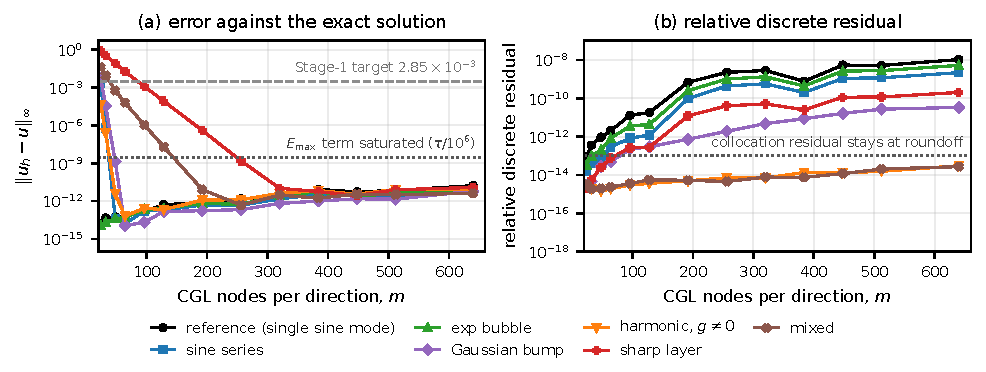
\includegraphics[width=0.92\textwidth]{../results/figures/convergence.pdf}
\caption{(a) Maximum error against the exact solution versus CGL resolution,
one representative case per family.  (b) Relative discrete residual over the
same runs: it stays at roundoff even when the solution error is large.}
\label{fig:conv}
\end{figure}

Stability of the direct solve was checked separately: for $24\le m\le640$ the
1-D spectra are real (zero imaginary part), the smallest denominator
$|\lambda_j+\mu_k|$ is $\approx19.7$, and $\kappa(V)$ grows only from $1.75$ to
$\condMax$.  No run produced a non-finite value and the finite-difference
fallback was never triggered.

\section{Runtime}

On a 4-core x86-64 laptop CPU (Python 3.14.8, numpy 2.5.4, reference OpenBLAS
3.12, no GPU) the Stage-1 reference case takes \runRef\,s.  An end-to-end run of
the official evaluator on one 12-case hidden-like suite --- one fresh process per
case, as in grading --- took \runMean\,s per case on average, $0.15$\,s at the
median, and \runMax\,s at worst (a sharp-layer case that exercises the full
$m=128,\dots,640$ schedule).  Over the \nCases-case sweep the median was
$0.18$\,s.  The official budget is $1200$\,s per case, so the solver uses about
$0.1\%$ of the allowance even in the worst case.  Cost is $O(m^3)$ for the
eigen-decomposition and the two transforms plus $O(Nm^2)$ for the barycentric
interpolation; runtime is set by the difficulty of the solution, not by the
output grid.

\section{Limitations and threats to validity}

\begin{itemize}
\item \textbf{Smoothness and geometry.} Exponential convergence holds for
  analytic data on a rectangle.  A jump in $f$ or $g$ would produce Gibbs
  oscillations that the difference-based adaptivity would report as
  non-convergence (the fallback is only second order), and general domains would
  need a different solver, e.g.\ a fast Poisson solver on a mapped domain.
\item \textbf{The residual is not an error certificate.} The collocation
  residual sits at roundoff even for inaccurate solutions, so adaptivity
  compares successive solutions rather than residuals; that comparison can in
  principle agree by accident, which is why we also enforce a minimum
  resolution.
\item \textbf{Benchmark scope.} The Stage-2/3 numbers come from manufactured
  solutions generated by the public case generator; real applications provide
  tabulated or noisy forcing, where interpolation of $f$ enters the budget.
  The proposal's PINN figures are used as published --- we did not retrain its
  $6\times50$ network --- so the comparison is operational, as the challenge
  specifies.
\item \textbf{Runtime and bit-level reproducibility.} Timings are from a
  4-core laptop; the grading machine may differ, but the margin to the
  20-minute limit is three orders of magnitude.  Bit-level results depend on
  the BLAS/LAPACK build: a clean venv from \texttt{requirements.txt} gives
  Stage-1 $\mathrm{MAE}=1.04\times10^{-12}$ instead of $2.93\times10^{-13}$,
  still far below every floor.
\end{itemize}

\section{Integrity statement}

The solver reads no files, uses no network, stores no answers, and never
branches on a case's name, family or index; $N$ is never assumed to be $129$
(tested for $N=33$--$513$, including descending grids).  Repeated runs are
bit-identical.  The hidden-like suites above come from the public
\texttt{hidden\_suite} generator with seeds we chose; the private seed was never
accessed.

\section*{References}
{\footnotesize
[1]~S. Malik, \emph{Physics-Informed Neural Network Shape Optimization}, GSoC 2026
proposal, ML4SCI, 2026 (benchmark and reported values).
[2]~M. Raissi, P. Perdikaris, G. E. Karniadakis, Physics-informed neural networks,
\emph{J. Comput. Phys.} 378 (2019) 686--707.
[3]~Z. Zhang, C. Lin, B. Wang, Physics-informed shape optimization using coordinate
projection, \emph{Sci. Rep.} 14 (2024) 6537.
[4]~L. N. Trefethen, \emph{Spectral Methods in MATLAB}, SIAM, 2000.
[5]~D. B. Haidvogel, T. A. Zang, The accurate solution of Poisson's equation by
expansion in Chebyshev polynomials, \emph{J. Comput. Phys.} 30 (1979) 167--180.
[6]~R. J. LeVeque, \emph{Finite Difference Methods for Ordinary and Partial
Differential Equations}, SIAM, 2007.
[7]~N. Kang et al., PIXEL: Physics-informed cell representations for fast and
accurate PDE solvers, \emph{AAAI} 37 (2023) 8186--8194; PIG: Physics-informed
Gaussians as adaptive parametric mesh representations, \emph{ICLR} 2025.
\par}

\end{document}
